\documentclass{article}
\usepackage{graphicx}
\usepackage{color}
\usepackage{calc}
\newsavebox\CBox
\newcommand\hcancel[2][0.5pt]{%
  \ifmmode\sbox\CBox{$#2$}\else\sbox\CBox{#2}\fi%
  \makebox[0pt][l]{\usebox\CBox}%  
  \rule[0.5\ht\CBox-#1/2]{\wd\CBox}{#1}}

\begin{document}
\section{Chapter 1}
\subsection{Exercises}
\subsubsection{Question 1.2}
\textbf{(a)} Absolute error $\approx 0.141592653$, the relative error $\approx 
4.507$ \%.


\textbf{(b)} Absolute error $\approx 0.001592653$, the relative error $\approx 
0.0506957$ \%.


\textbf{(c)} Absolute error $\approx 0.001264489$, relative error $\approx 
0.0402499$ \%.

\subsubsection{Question 1.5}

The condition number is defined as follows:
$$Cond = \frac{|(f(\hat{x}) - f(x))/f(x)|}{|(\hat{x}-x)/x|}$$

but more carefully:
$$Cond = \frac{|((x + \Delta x)-(y + \Delta y)) - \textcolor{blue}{(x-y)}|/|
\textcolor{red}{x-y}|}{|(|x + \Delta x| + |y + \Delta y|)-(\textcolor{blue}{|x| + 
|y|})|/(\textcolor{red}{|x| + |y|)}}$$
$$\geq \frac{|(\hcancel{(x - y)}\textcolor{blue}{\epsilon} + \Delta x - \Delta y) 
- \textcolor{blue}{\epsilon}|/|\textcolor{red}{\epsilon}|}{|(\hcancel{|x| - |x|} + 
|\Delta x| + \hcancel{|y | - | y|} + \Delta y|)|/(\textcolor{red}{1})}$$

$$ = \frac{|\Delta x - \Delta y| /\epsilon}{(|\Delta x| + |\Delta y|)/1} $$
$$ \geq \frac{1}{\epsilon} $$

The condition number is therefore necessarily larger than $\frac{1}{\epsilon}$, 
which means as $\epsilon$ gets closer to 0, we have more sensitivity in $f$. Since 
$x-y \approx \epsilon$, this means that the function gets more sensitive the 
closer $x$ and $y$ are to each other in value.

\subsubsection{Question 1.6}
Forward error is $\hat{f}(x)-f(x)$, and the backward error is $\hat{x} - x$ where 
$f(\hat{x}) = \hat{f}(x)$.


\textbf{(a)}

\textit{x=0.1}: The forward error is $$0.1 - sin(0.1) = 1.665*10^{-4},$$
the backward error is $$\hat{x} -x = sin^{-1}(0.1) -0.1 = 0.100167 - 0.1 = 
1.67*10^{-4}.$$


\textit{x=0.5}: The forward error is $$0.5 - sin(0.5) = 0.0205,$$ the backward 
error is
$$\hat{x} -x = sin^{-1}(0.5) - 0.5 = 2.36 * 10^{-2}.$$


\textit{x=1.0}: The forward error is $$1 - sin(1) = 0.1585,$$ and the backward 
error is $$\hat{x}-x=sin^{-1}(1) - 1 = 0.5708.$$

\textbf{(b)}
In this case, the forward error is $$\hat{f}(x) - f(x) = x-\frac{x^{3}}{6} - 
sin(x),$$
and the backward error can be found using the following:
$$backerr = \hat{x} - x,$$
where

$$\hat{x} = f^{-1}(\hat{f}(x)) = arcsin(x - \frac{x^{3}}{6}),$$

\textit{x=0.1}: The forward error is $$0.1-\frac{(0.1)^{3}}{6} - sin(0.1)= 
-8.331*10^{-8},$$ and the backward error is $$x - \hat{x} = 0.1 - arcsin(0.1 - 
\frac{0.1^3}{6} = 0.000000083731.$$

\textit{x=0.5}: The forward error is $$0.5-\frac{(0.5)^{3}}{6} - sin(0.5)= 
-2.588*10^{-4},$$  and the backward error is $$x - \hat{x} = 0.5 - arcsin(0.5 - 
\frac{0.5^3}{6} = 0.00029495.$$

\textit{x=1.0}: The forward error is $$1.0-\frac{(1.0)^{3}}{6}- sin(1.0) = 
-8.137*10^{-3},$$ and the backward error is $$x - \hat{x} = 1.0 - arcsin(1.0 - 
\frac{1.0^3}{6} = 0.0148892.$$

\subsubsection{Question 1.10}

\paragraph{\textbf{(a)} For x values near 0.}
\paragraph{\textbf{(b)} The following is more stable around x = 0 because any 
rounding errors only occur once.
$$\frac{1}{1-x} - \frac{1}{1+x} = \frac{2x}{1- x^2}$$}


\subsubsection{Question 1.22}
Assume a normalized floating-point system with $\beta{} = 10$, $t = 3$, and
$L = -98$.

\paragraph{(a)}
$$UFL = \beta{}^{l} = 10 ^{-98}$$

\paragraph{(b)} If $x = 6.87 × 10^{-97}$ and $y = 6.81 × 10^{-97}$ ,
what is the result of $x - y$?\\

Ignoring the system, $x - y = 0.06 * 10 ^{-97}$ which if we normalize (which in 
the initial case we must), we have the result = $6*10^{-99}$ which is smaller than 
the underflow value. If we're assuming truncation, then we end up with a value of 
0 for this result.



\paragraph{(c)}What would be the result of $x - y$ if the
system permitted gradual underflow?

If the system permitted gradual underflow, then the result would be

$$result= 0.60 * 10^{-98}.$$


\subsection{Computer Exercises}
\subsubsection{Question 1.6}

\textbf{(a)}The method which uses multiplication, ie

$$x_k = a + kh, \qquad k=0,...,n$$

is better than the recursive summation method. Since we are using floating
point arithmetic, every step of the recursive method will involve some rounding. 
This loss of precision (error) will accumulate in the sum. While the 
multiplicative method also involves rounding, there are only two opperations, so 
the loss of precision is restricted to whatever occurs because of those two 
operations. Basically there are two rounding errors for the multiplicative method 
while the recursive method adds $n$ rounding errors.

\textbf{(b)}
In order to do this we set $a=0$, $b=1$ and use $n=10000$. We computed the $x_k$ 
for both methods and compared the results by taking the squared error between each 
term of each method and a true set of values achieved using $np.linspace$. The 
code can be found in $assignment1.ipynb.$\\

\begin{figure}
	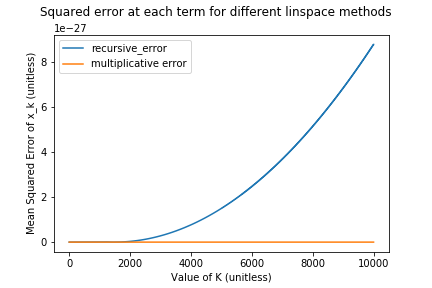
\includegraphics[width=\textwidth]{fig_ch1_cp1_6.png}
	\label{fig:ch1_cp1_6}
	\caption{Comparison of the error of the two proposed linspace generation 
	methods.}
\end{figure}

\subsubsection{Question 1.7}

\begin{figure}
	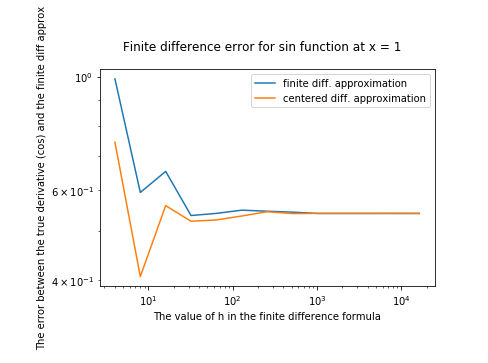
\includegraphics[width=\textwidth]{finite_diff_error_plot.png}
	\label{fig:ch1cp17}
	\caption{Plot of the errors for the finite difference and centered
	 difference approximations of the derivative of sin(x) at x = 1.0
	  for different values of h.}
\end{figure}

There isn't really much to comment about for this question. The plot 
requested can be found in figure \ref{fig:ch1cp17}. Appart from that 
you can find the code in $assignment1.ipynb.$\\




\subsubsection{Question 1.9}

\paragraph{(a)} The code for this question can be found in $assignment1.ipynb.$

\paragraph{(b)} The natural way to stop is when the term we are adding hits the value of 0. This is because factorials grow faster than their equivalent polynomials, so at one point the denominator will be so much bigger than the numerator that it will round to zero in the computer.

\paragraph{(c)} The results are shown in figure \ref{fig:q19}


\begin{figure}
	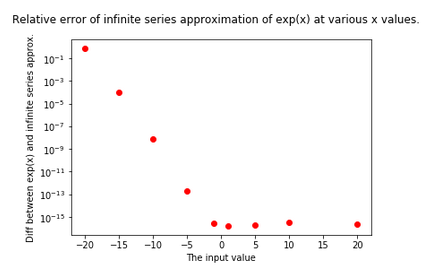
\includegraphics[width=\textwidth]{exp_infinite_series.png}
	\label{fig:q19}
	\caption{Plot of the relative error of the infinite series approximation
	of the exponential function.}
\end{figure}

\subsubsection{Question 1.10}

\subsubsection{Question 1.14}


\iffalse
\section{Chapter 2}
\subsection{Exercises}
\subsubsection{Question 2.7}
\subsubsection{Question 2.13}
\subsubsection{Question 2.21}
\subsubsection{Question 2.22}
\subsubsection{Question 2.32}
\subsubsection{Question 2.37}
\subsection{Computer Exercises}
\subsubsection{Question 2.5}
\subsubsection{Question 2.6}
\subsubsection{Question 2.9}
\subsubsection{Question 2.11}
\subsubsection{Question 2.17}
\fi
\end{document}
